% \subsection{Characterization of Performance}

Before embarking on a computational campaign that will consume 150M core
hours on the NCSA Blue Waters machine, we study the scalability of HTBAC so
as to determine optimal workflow sizing and resource utilization for the
ESMAC protocol. The goal is twofold: (1) understanding the invariance of
HTBAC execution time over the number of workflow pipelines executed; and (2)
studying how the performance of EnTK and RP varies in relation to the size of
workflow.

% ---------------------------------------------------------------------------
\subsubsection{Experiment Design}\label{ssec:exp_design}

We designed two experiments to measure HTBAC, EnTK and RP weak scalability
when executing an increasing number of concurrent pipelines. According to the
use case described in Section~\ref{sec:htbac}, each pipeline consists of
seven stages, each stage with a single task. EnTK manages the queuing of the
tasks in accordance with the order and concurrency mandated by stages and
pipelines: For each pipeline, each stage is executed sequentially while
pipelines are executed concurrently.

Experiment 1 measures the baseline behavior of EnTK and RP with the workflow
of the ESMACS protocol and a null workload (\textmd{/bin/sleep 0}). The goal
is to isolate the overheads of EnTK and RP from the specifics of the
executables of the workflow and the overheads of the resources. The null
workload does not require data staging, I/O on both memory and disk, or
communication over network.

Experiment 2 replicates the design of Experiment 1 but it executes the
workflow of the ESMAC protocol with the actual simulation and data workload.
The comparison between the two experiments enables performance analysis of
EnTK and RP to understand whether and how the size of the executed workflow
affects its overheads. Further, Experiment 2 shows also whether HTBAC
execution time is sensitive to the number of concurrent pipelines executed.

Both experiments measure the weak scalability of HTBAC, EnTK and RP\@. This
means that the ratio between the number of pipelines and cores is kept
constant by design. While an investigation of strong scalability would
contribute to a better understanding of the behavior of HTBAC, EnTK and RP,
it is of limited interest for the current use case. The driving goal of HTBAC
is to increase throughput by a means of concurrency of pipelines, not in the
number of sequential executions per core. This is a driving motivation to
target large HPC machines instead of so-called HTC infrastructures.

% ---------------------------------------------------------------------------
\subsubsection{Experiment Setup}\label{ssec:exp_setup}

We perform both Experiment 1 and 2 on NCSA's Blue Waters---a 13.3 petaFLOPS
Cray, with 32 Interlago cores/50 GB RAM per node, Cray Gemini, Lustre shared
file system. Currently, we exclusively use CPUs on Blue Waters as GPUs are
not required by our use case. RCT support the use of both type of
architectures and we previously benchmarked the use of GPUs.

We perform our experiments from a virtual machine hosted in Europe. This
helps to simulate the conditions in which the experimental campaign will be
performed by the research group at UCL\@. This is relevant because, as most
HPC resources, Blue Waters does not allow for executing applications on the
login node of the cluster. To this end, RCTs support \textmd{gsissh} for X509
authentication and authorization.

Table~\ref{tab:exp} shows the setup for Experiment 1 and 2. The ESMACS
protocol is executed with up to 25 concurrent but independent pipelines and
therefore their concurrent execution does not entail communication overhead.
Further, the system simulated can benefit from concurrency because potential
HTBAC users may wish to extend their protocols beyond the current scale of
ESMACS\@. Consistently, our experiments push the boundaries of current scale
by executing 8, 16, 32, 64 and 128 concurrent pipelines.

\begin{table*}[t]
\centering
\caption{\bf Experiment 1 executes the 7 stages of the ESMACS protocol with
a null workload; Experiment 2 uses the actual workload of the ESMACS
protocol. ESMACS protocol with NAMD and supporting workload: (1) Untar
configuration files; (2) Preprep; (3) Minimize with decreasing restraints;
(4) Equilibration: NVT simulation at 50K, with restraints; (5) Equilibration:
NPT simulation at 300K, with decreasing restraints; (6) Equilibration: NPT at
300k, no constraints; (7) Tarball output files.}\label{tab:exp}
\begin{tabular}{llllllll}
\toprule
\textbf{Experiment ID} & 
\textbf{Protocol}      & 
\textbf{Workload}      & 
\textbf{Trials}        & 
\textbf{Pipelines}     & 
\textbf{Stages}        & 
\textbf{Tasks}         & 
\textbf{Cores} \\ 
\toprule
1 & ESMACS & Null workload & 2 & 8, 16, 32, 64, 128 & 7 & 7 & 64, 128, 256, 512, 1024\\ 
2 & ESMACS & (NAMD and Supporting Workload) & 2 & 8, 16, 32, 64, 128 & 7 & 7 & 64, 128, 256, 512, 1024 \\ 
\bottomrule
\end{tabular}
\end{table*}

EnTK uses RADICAL-Pilot to acquire resources via a single pilot. The size of
the pilot is contingent upon characterization of performance, in this case,
weak scalability. Accordingly, we use the same number of cores in a pilot as
those required by the workload. We use between 64 and 1024 cores in both
Experiment 1 and 2. \jhanote{Following needs fixing before it can be
reinserted: and we always keep the number of simulations equal to the number
of cores.} We use either 1 or 8 cores per task depending on the task
requirements.

% \mtnote{The following needs discussion: ``The size of the workload is
% varied in proportion to the amount of resources such that all tasks are
% concurrently executed at all times.'' I believe this is not necessary true:
% we do not execute all the tasks concurrently all the time but we always get
% enough cores to run at least one task from each concurrent pipeline.
% Alternatively, at every point in time, there are enough cores so that
% pipelines do not compete for the same core.}\jhanote{I agree we do not run
% all the tasks concurrently.}

% \mtnote{I would represent the following with a table. Please feel free to
% change it back if you disagree. ``For example, in the ESMACS protocol, the
% simulation task specifies 8 cores per pipeline, therefore the pilot size is
% defined as 8 \(\times \) number of pipelines. We vary the number of
% pipelines to characterize weak scaling performance where the tasks are
% scheduled concurrently.''}

% \mtnote{The following should probably moved to the next subsection, when
% discussing the results of the experiments: ``For each of these
% configurations, the simulation execution time is observed to be
% constant.''}
% \jhanote{yes}

All the experiments use Ensemble Toolkit version 0.4.7 and RADICAL-Pilot
version 0.42. The MD engine used is NAMD-MPI\@. The equilibration % stages 
tasks of stage 4 and 6 are assigned 5000 timesteps while the task of stage 5
requires 55000 timesteps. We ran both the null and MD workload for two trials
at each pipeline configurations.

% ---------------------------------------------------------------------------
\subsubsection{Results}\label{ssec:exp_results}

First we characterize the overhead of RADICAL-Pilot (RP) and EnTK in the 
null workload, where we isolate the % any 
overhead introduced by the two % application
systems (Figure~\ref{fig:exp1}). We see a (slightly) superliner
increase of EnTK overhead, between 0.1 and 1.8 seconds. This overhead depends
on the number of tasks that need to be translated in-memory from a Python
object to a compute unit (CU) description. As such, it is expected to grow
proportionally to the number of tasks, barring some competition of resources.

% on a shared workstation like the one used for our experiments.

\begin{figure}
  \centering
  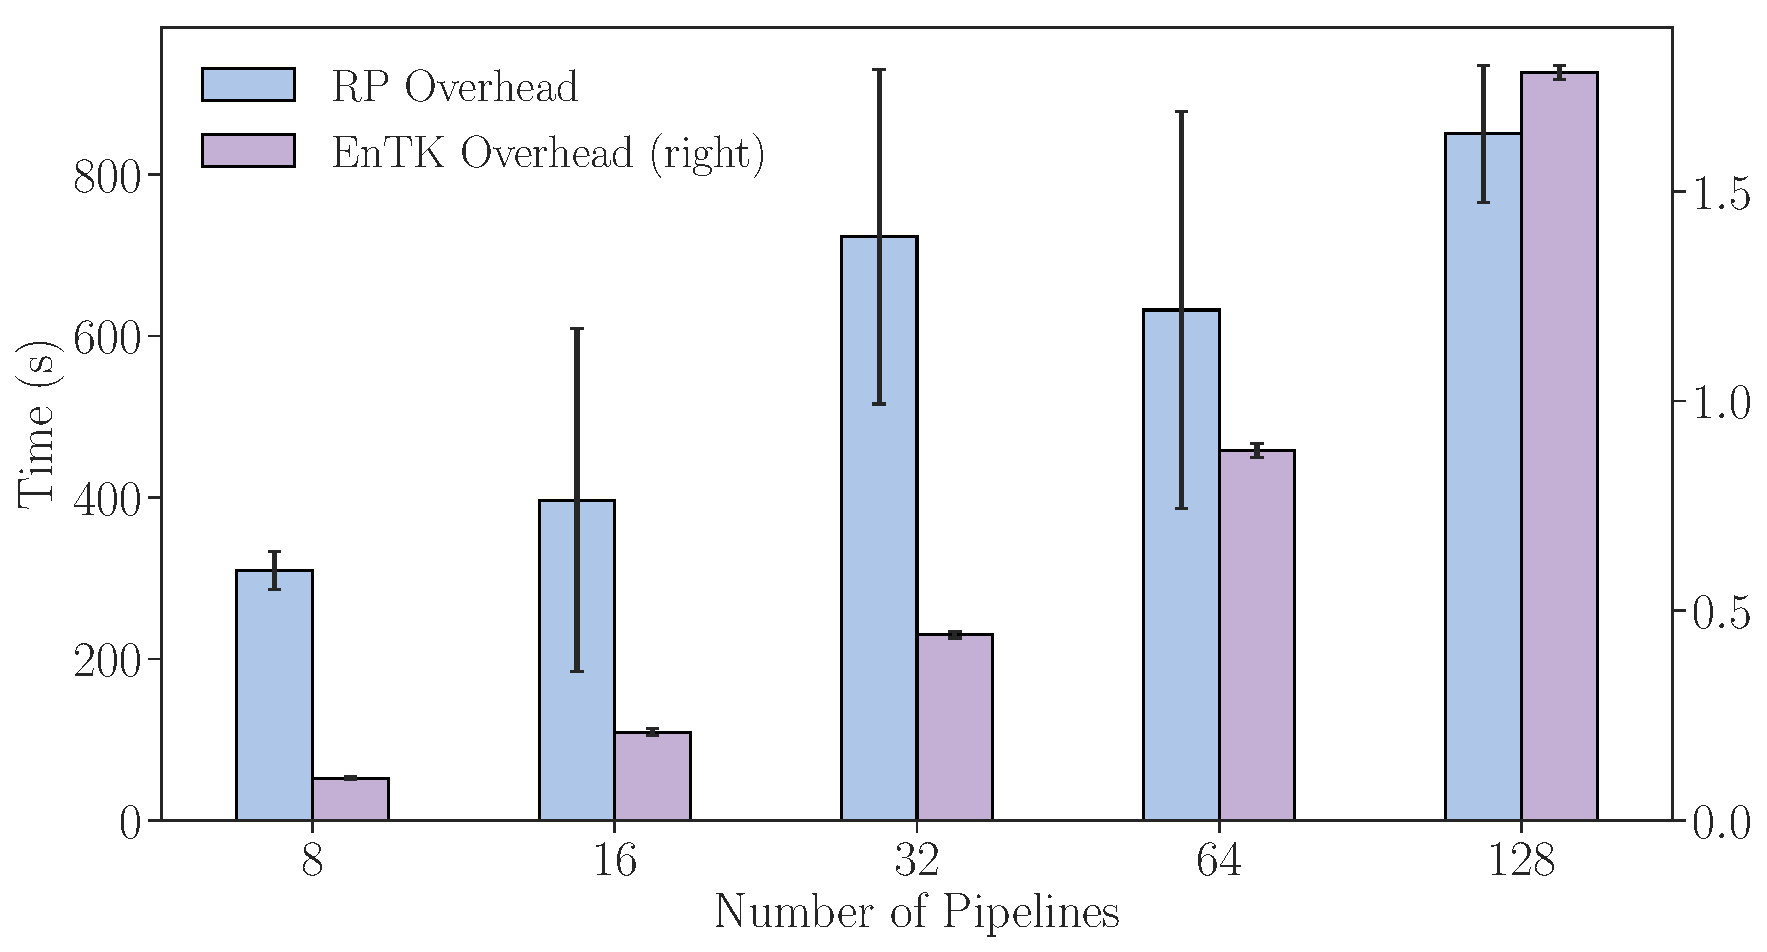
\includegraphics[width=\columnwidth]{FIGURES/null_workload_overheads.pdf}
  \caption{Overheads of Ensemble Toolkit (EnTK) and RADICAL-Pilot (RP) when
           executing HTBAC using a null workload. We plot the baseline
           EnTK/RP overheads without the application workload across two
           trials per pipeline configuration.}\label{fig:exp1}
\end{figure}

% Weak scaling of HTBAC using null workload. We observe similar behavior at
% each configuration in the simulation execution time showing that the EnTK
% is invariant to the workload and a steady increase in the RP overhead due
% to the increase in the number of stages

RP overhead is also, on average, superlinear but with a much greater
variance. This variance is due to mainly two factors: Network latency and
filesystem latency on the HPC resource. EnTK submits CU descriptions to the
MongoDB used by RP, and RP pilot pulls these descriptions from the same
database. As described in Section~\ref{ssec:exp_setup}, this pull operation
occurs over a wide area network, introducing varying amount of latency.
Further, RP pilot writes and reads the CU descriptions multiple times to
and from the shared filesystem of the HPC machine. Together, these two
factors introduce delays in the scheduling of the CUs.

% We see a steady superlinear increase in the RP and EnTK overheads as we
% grow the number of pipelines. Note that the RP overhead also captures the
% overhead introduced by the Blue Waters file system, network communication,
% time to stage the units and communication to the database.

When the workload is the EGFR kinase, we see (Figure~\ref{fig:exp2}) that the RP
overhead becomes on average less than 10\% of the average total execution time
(TTX), defined as \(TTX = TTC - T_q\) where \(TTC\) is time-to-completion and
\(T_q\)% where we measure TTX as 
is time spent queuing on the HPC machine. We notice the TTX is essentially
invariant 
across pipelines of different size and that, when accounting for variance, RP
overheads also shows linear weak scaling behavior. As expected, EnTK overhead
remains superlinear and comparable to the one measured in Experiment 1. This
is because in both experiments EnTK overhead depends on the number of tasks
translated to CU descriptions.

\begin{figure}
  \centering
  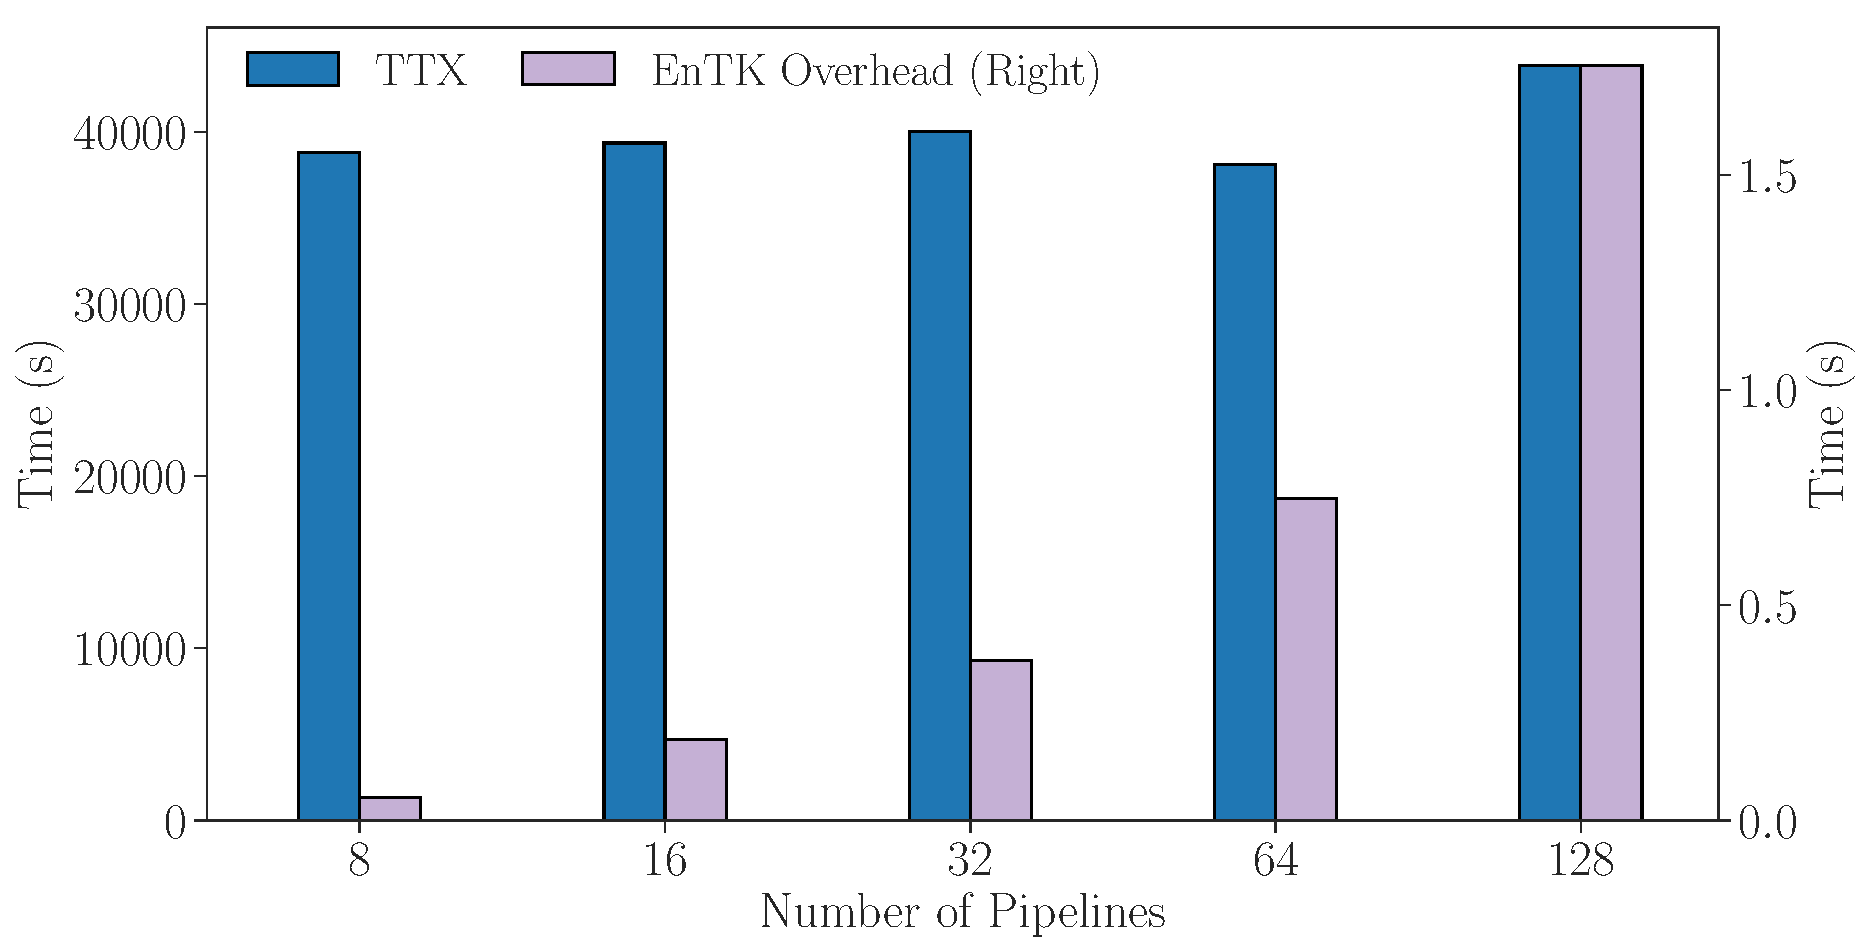
\includegraphics[width=\columnwidth]{FIGURES/namd_workload_overheads.pdf}
  \caption{Introducing the use-case NAMD and supporting workload, we observe
  similar EnTK/RP overhead behavior as with the null workload with higher
  values as the number of pipelines increases. Across pipeline
  configurations, TTX and RP overheads (accounting for the error bars) show % a correct trend in 
  weak scaling performance.}\label{fig:exp2}
\end{figure}

% Weak scaling of HTBAC using use-case payload. We observe higher
% time-to-completions for each  than the null workload yet similar
% performance across pipelines indicating optimal weak scaling
% characterization

Experiments 1 and 2 show how the overheads of both EnTK and RP tend to be
invariant across type of workload executed. Their scaling behavior and, to
some approximation, their absolute values are comparable between
Figure~\ref{fig:exp1} and~\ref{fig:exp2}. This is relevant because it shows
that the systems used to coordinate and execute the ESMACS protocol add a
constant and comparatively not relevant overhead to the execution of NAMD\@.

% In both payloads, the RP and EnTK overheads showed an invariance to
% the type of payload.

% Moreover we validate the concurrency in the execution of tasks based on the
% performance of weak scaling in the use-case workload where the execution
% time (TTX) behaves similarly as the pipeline configuration is increased.

% The RP overhead demonstrates the core overhead which is the
% time-to-completion (TTC) as measured by RADICAL Pilot as well as the Blue
% Waters file system overhead, network communication, time to stage the
% units, and the latency of communication to the database.

% For the NAMD workload, we show weak scaling results for the overheads and
% the simulation execution time which corresponds to the time taken by all
% the simulations to complete.

% The fluctuation of the simulation execution times can be attributed to
% run-time system fluctuations within the workload including stragglers at
% higher pipeline and pipeline-to-pipeline fluctuations. In order to examine
% the fluctuations within stages we correlate the overhead for each pipeline
% at the longest simulation duration in order to reconcile any fluctuations
% induced by NAMD\@. We calculate time-to-execution (Tx) of the largest
% pipeline size and compare the longest MD run within each pipeline. The NAMD
% logs indicate a mean and variance as\ldots

% \begin{figure}[!htbp]
%   \centering
%   %\begin{minipage}[b]{0.6\textwidth}
%   \begin{minipage}[b]{0.55\textwidth}
%   \centering
%   %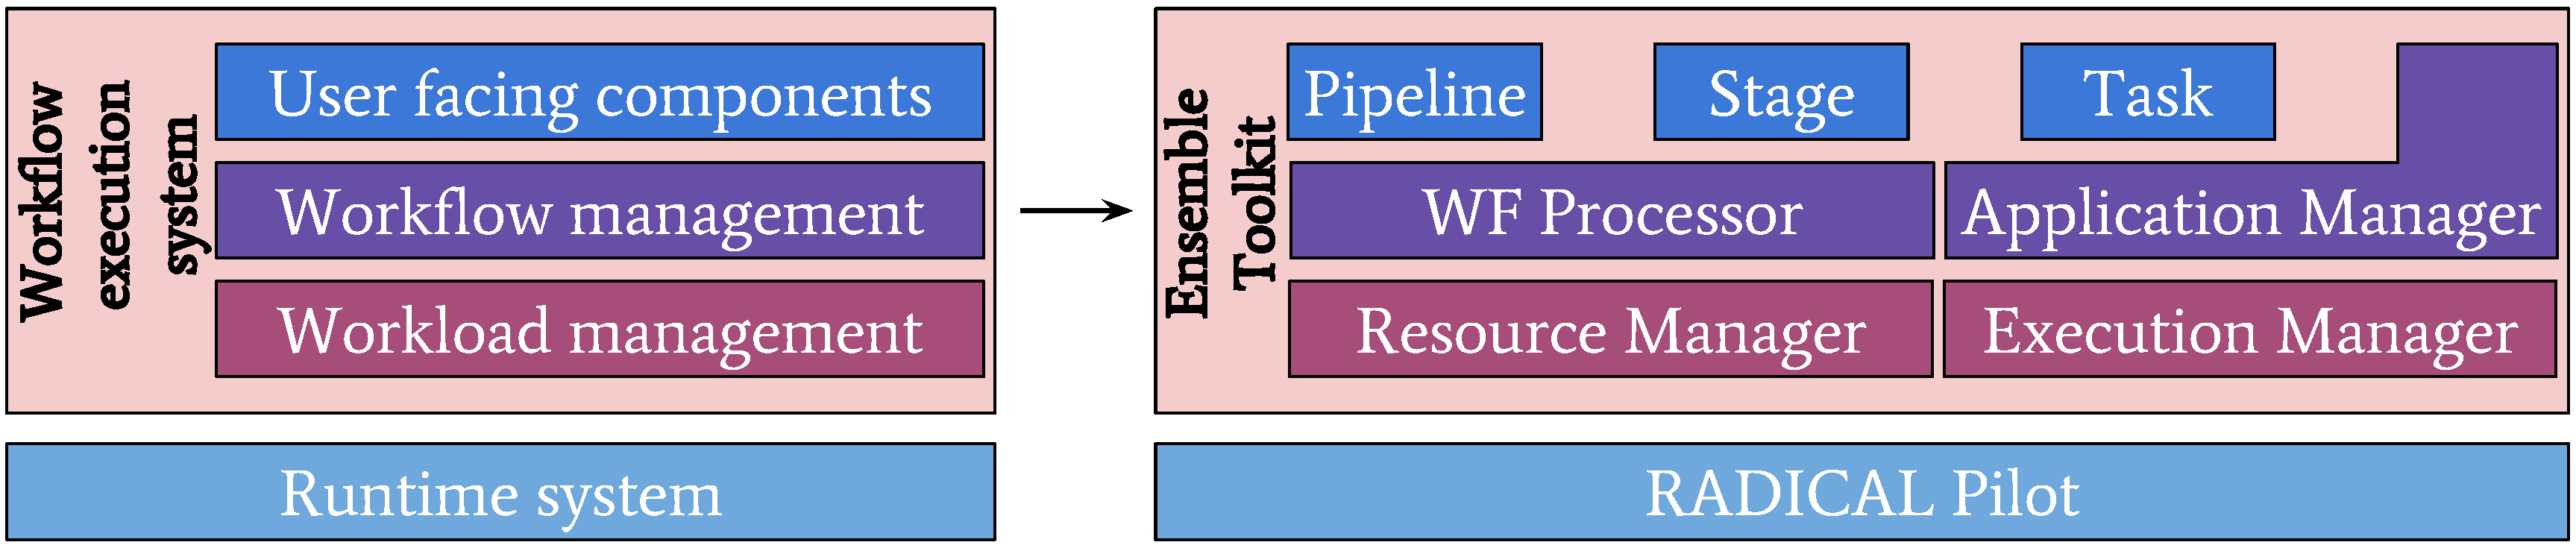
\includegraphics[width=\textwidth, height=35mm]{FIGURES/entk_overview.pdf}
% %  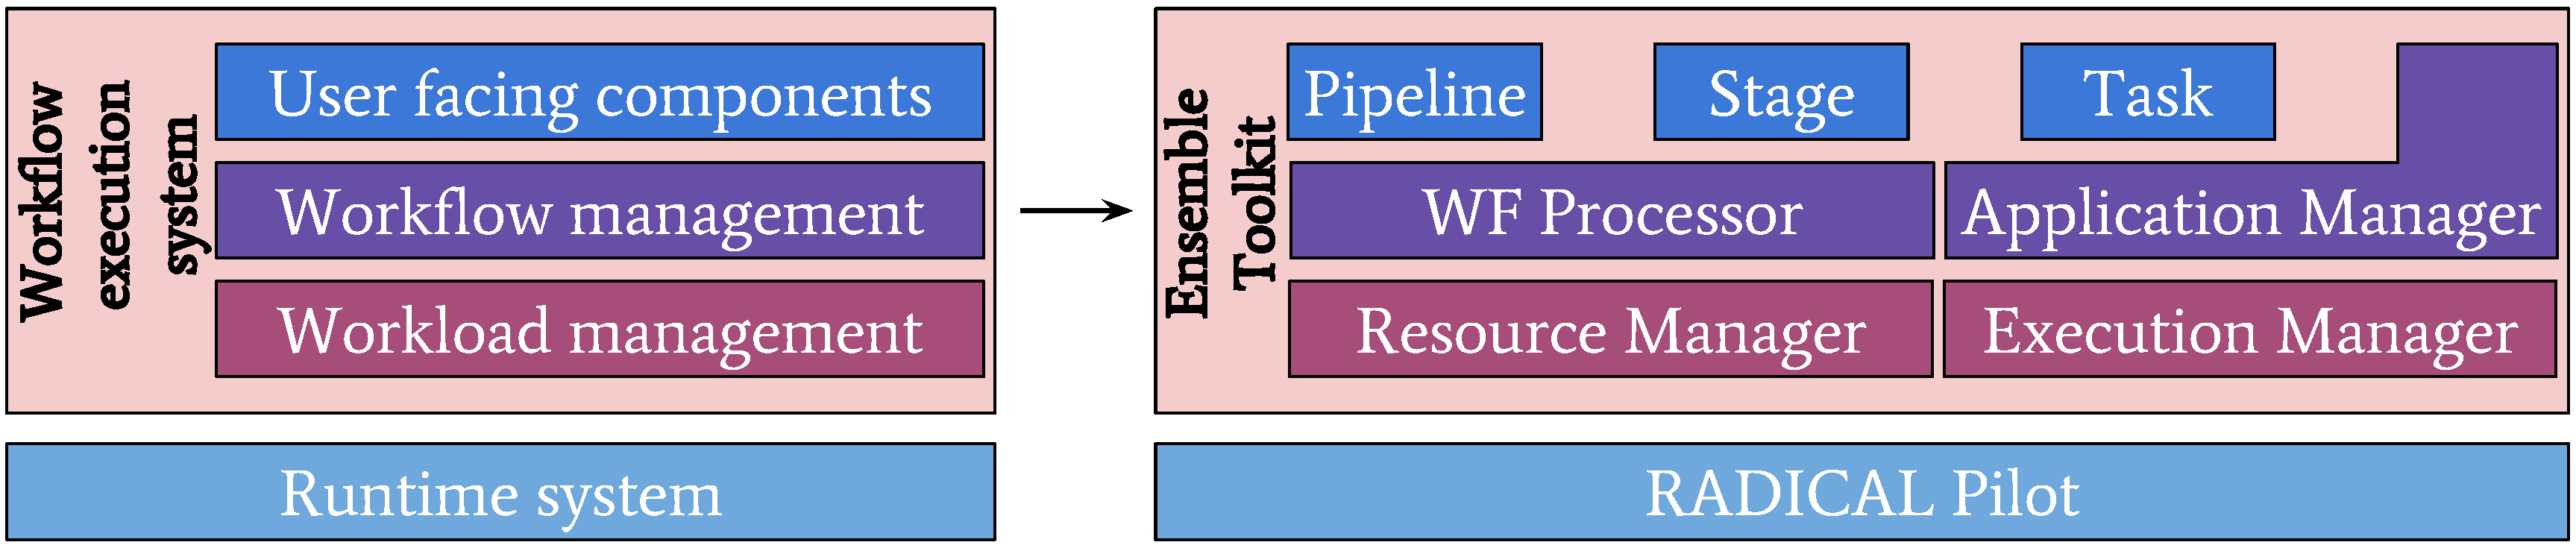
\includegraphics[width=\textwidth, height=40mm]{FIGURES/entk_overview.pdf}
%   \end{minipage}
%   %\begin{minipage}[b]{0.39\textwidth}
%   \begin{minipage}[b]{0.44\textwidth}
%   \centering
% %  \includegraphics[width=\textwidth, height=35mm]{FIGURES/md_general.pdf}
% %  \includegraphics[width=\textwidth, height=40mm]{FIGURES/md_general.pdf}
%   \end{minipage}
%   \caption{Overview of time-to-execution (Tx) of each pipeline at the
%            longest simulation duration as measured by NAMD log files,
%            showing how the distribution shows no abnormal fluctuations
%            across pipelines.}\label{fig:namd_logs}
% \end{figure}

% \begin{figure}[!htbp]
%   \begin{minipage}[b]{0.49\textwidth}
%   \centering
%   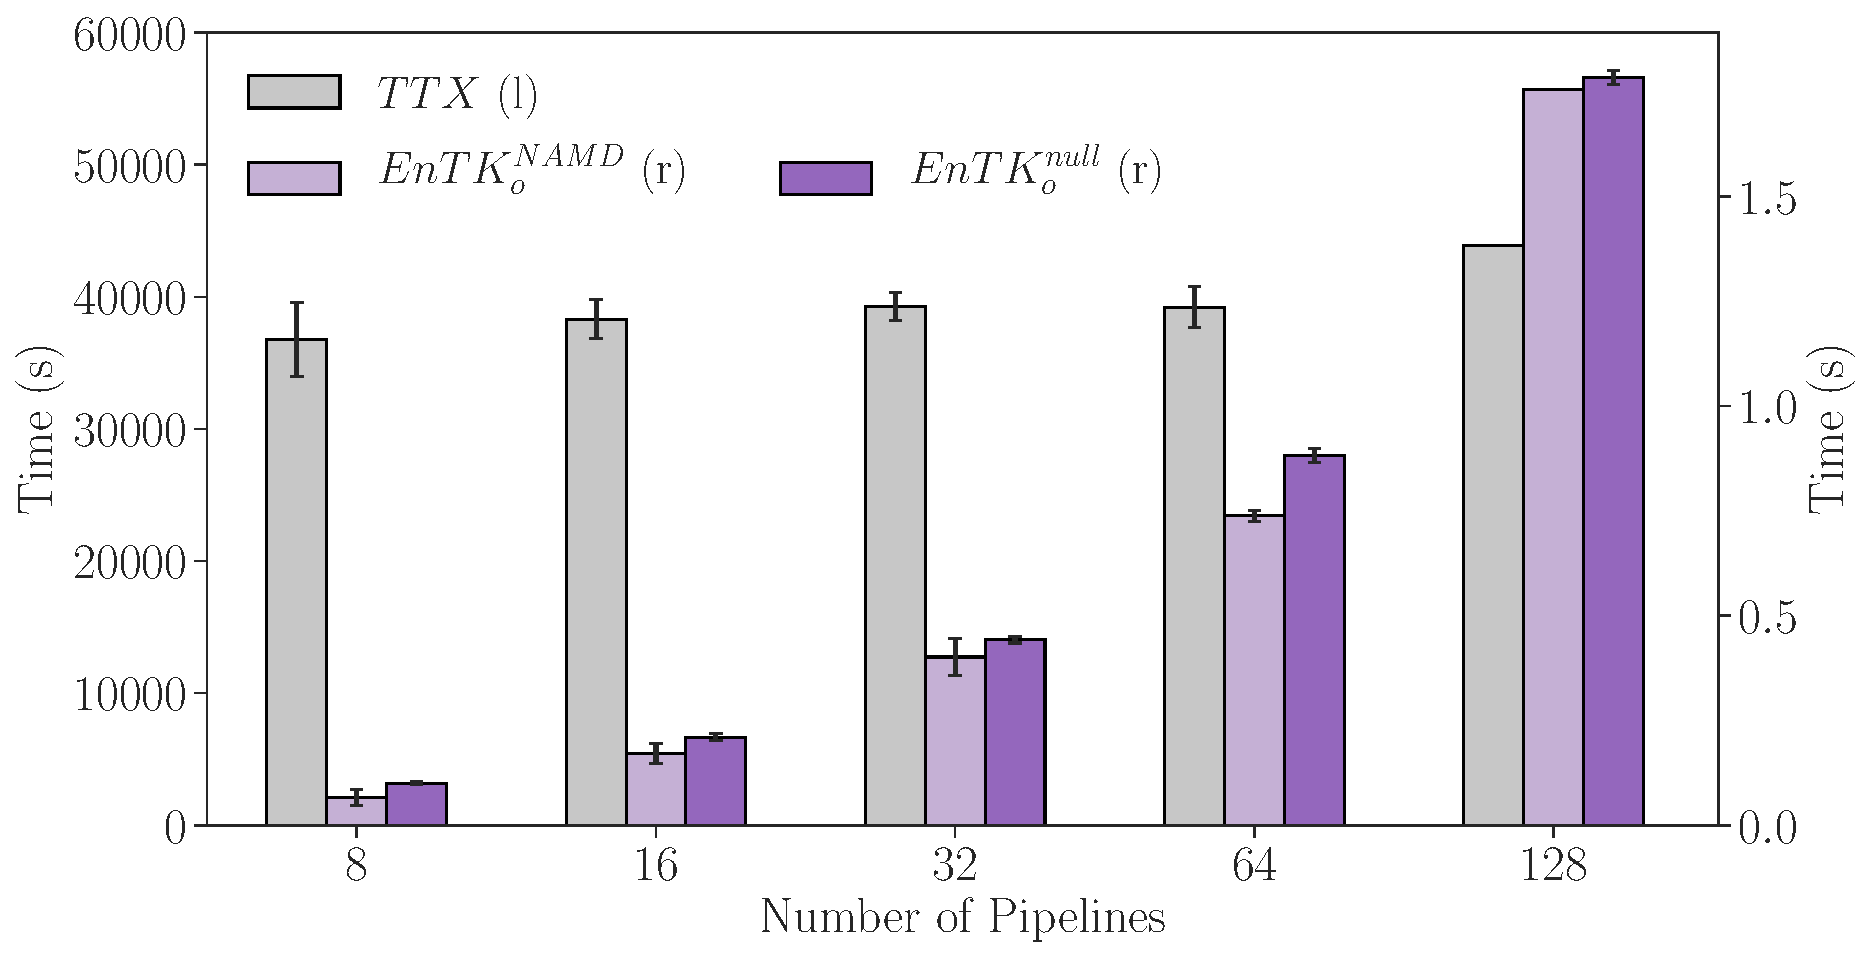
\includegraphics[width=\textwidth]{FIGURES/namd_null_workload_overheads.pdf}
%   \end{minipage}
%   \caption{EnTK overheads for null and NAMD workflows; no pilot overheads.}\label{fig:namd_logs}
% \end{figure}


% NAMD logs - corrolate the overhead for each pipeline makes the system
% invariant to the worload. Remaining will be RP overhead. NAMD log files
% (utime) demonstrates time-to-execution (Tx)

%Add in: what are the overheads, how is EnTK collecting overhead 




%eq0 : Minimize with decreasing restraints
%eq1 : NVT, 50K, with restraints
%eq2 : NPT, 300K, with decreasing restraints 
%sim1.conf: NPT, 300k, no constraints


%Need system verification of timestamps (errors) 




